\chapter{Continental}\label{chapConti}
\putminitoc
J'effectue mon stage au sein de l'entreprise Continental, une entreprise ayant pris une très grande importance dans le monde de l'automobile. 

Afin de vous présenter le contexte dans lequel j'ai travaillé, nous allons voir comment opère cette société, et plus particulièrement l'équipe dans laquelle j'ai travaillé : l'équipe \textit{Tests \& Automation Service}.

	\section{Organisation de l'entreprise}
		\subsection{Continental AG}

Continental AG est une entreprise allemande fondée en 1871 dont le siège se situe à Hanovre. Il s'agit d'une Société Anonyme (SA) dont le président du comité de
direction est le Dr. Elmar \bsc{Degenhart} depuis le 12 août 2009. Elle est structurée autour de deux grands groupes : le groupe Rubber et le groupe Automotive.
	 
		 \begin{figure}[H]
		 	\centering
		 	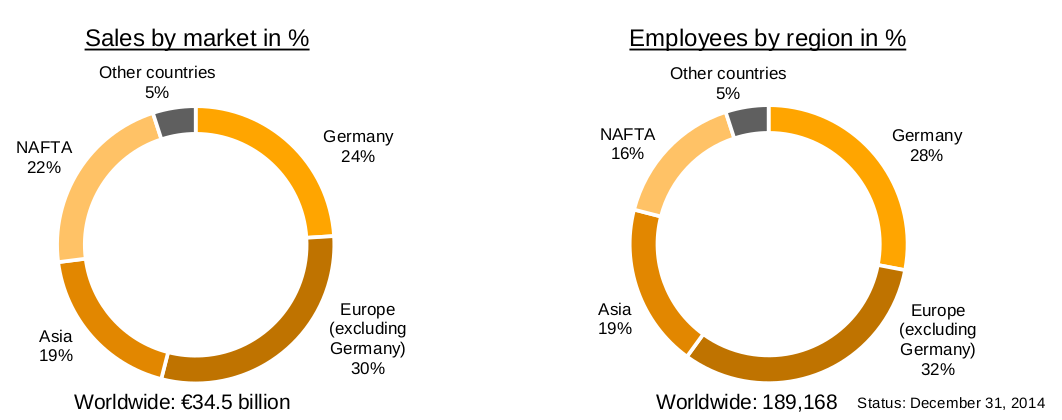
\includegraphics[width=19cm]{contents/images/caConti.png}
		 	\caption{Chiffre d'affaire et nombre d'employés (Année 2014)}
		 	\label{fig:caConti}
		 \end{figure}

		 En 2014, l'entreprise comptait plus de $189\;000$ employés dans le monde\footnote{Cf figure \ref{fig:caConti}} répartis dans 317 sites et 50 pays différents\footnote{Cf figure \ref{fig:repartitionConti}}. Avec un chiffre d'affaire de 34.5 milliards d'euros au total, Continental est le numéro un du marché de production de pneus en Allemagne et est également un important équipementier automobile.
		 \begin{figure}[H]
		 	\centering
		 	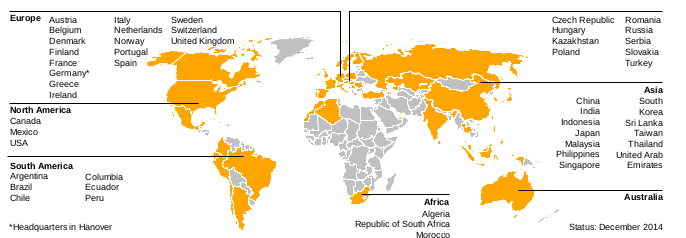
\includegraphics[width=18cm]{contents/images/repartitionConti.png}
		 	\caption{Répartition du groupe Continental dans le monde}
		 	\label{fig:repartitionConti}
		 \end{figure}		 

		\subsection{Histoire de l'entreprise}
		Continental est fondée en 1871 comme société anonyme sous le nom de <<\textit{Continental-Caoutchouc-und Gutta-Percha Compagnie}>> par neuf banquiers et industriels de Hanovre (Allemagne).

		Continental dépose l'emblème du cheval représenté sur la figure \ref{fig:logo}, comme marque de fabrique à l'Office impérial des brevets de Hanovre en octobre 1882. Ce logo est aujourd'hui encore protégé en tant que marque distinctive.
		\begin{figure}[H]
			\centering
			
\includegraphics[width=3cm]{contents/images/logoConti.png}
			\caption{Logo de Continental}
			\label{fig:logo}
		\end{figure}

		Le fabricant de pneus allemand débute son expansion à l'international en tant que sous-traitant automobile international en 1979, expansion qu'il n'a cessé de poursuivre depuis.
		
Entre 1979 et 1985, Continental procède à plusieurs rachats qui permettent son essor en Europe, celui des activités pneumatiques européennes de l'américain \textit{Uniroyal Inc.} et celui de l'autrichien \textit{Semperit}.

En 1995 est créée la division << \textit{Automotive Systems} >> pour intensifier les activités << systèmes >> de son industrie automobile.

La fin des années 1990 marque l'implantation de Continental en Amérique latine et en Europe de l'Est.

En 2001, pour renforcer sa position sur les marchés américain et asiatique, l'entreprise fait l'acquisition du spécialiste international de l'électronique \textit{Temic}, qui dispose de sites de production en Amérique et en Asie. La même année, la compagnie reprend la majorité des parts de deux entreprises japonaises productrices de composants d'actionnement des freins et de freins à disques. 

En 2004, le plus grand spécialiste mondial de la technologie du caoutchouc et des plastiques naît de la fusion entre \textit{Phoenix AG} et \textit{Conti'Tech}.

Enfin en juillet 2007, Continental réalise sa plus grosse opération en rachetant le fournisseur automobile \textit{Siemens VDO Automotive}. Ce rachat a permis à l'entreprise de multiplier son chiffre d'affaire par deux, passant ainsi de 13 milliards d'euros à plus de 30.5 milliards d'euros (chiffre de 2014).
		
		\subsection{Activités des différentes branches}
		\begin{figure}[H]
			\centering
			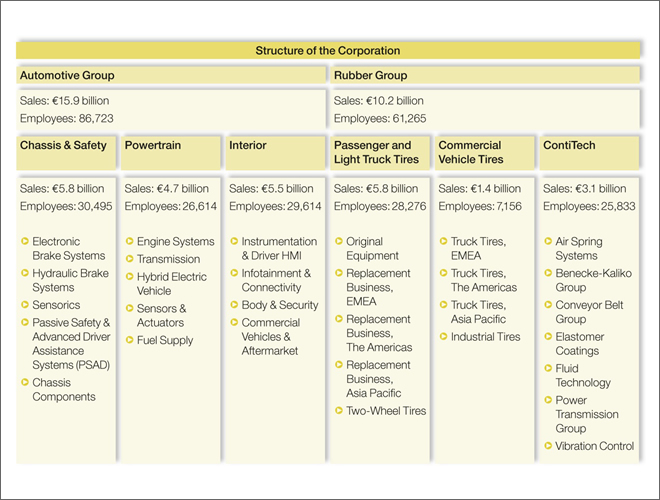
\includegraphics[width=18cm]{contents/images/structureConti.jpg}
			\caption{Structure de Continental}
			\label{fig:structConti}
		\end{figure}

		Comme on peut le voir sur la figure \ref{fig:structConti}, Continental est composée de deux groupes et de six divisions. Ces dernières se chargent de développer et produire des équipements répondant aux besoins des clients. Pour cela elles sont composées de \textit{Business Units} qui ont chacune une activité bien particulière dans leur domaine de compétence. 

Durant mon stage, je travaillais au sein de \textit{P-ES} : division \textit{Powertrain} et \textit{Business Unit} \textit{Engine Systems}. Elle s'occupe essentiellement du contrôle moteur, au niveau logiciel et matériel avec l'ECU\footnote{Electronic Control Unit} et de la mise au point des systèmes diesel et essence. La BU \textit{Engine Systems} est quant à elle chargée de produire les équipements nécessaires au contrôle moteur tels que des calculateurs ou des injecteurs.

	\section{Le contexte de l'équipe TAS}
 		\subsection{L'équipe Tests \& Automation Service}
 		J'ai travaillé dans l'équipe en charge des tests au niveau système ou logiciel dirigée par Corinne \bsc{Tarin}. 
 		% P : Powertrain
 		% ES : Engine System
 		% SE :
 		% CV :
	 	% TAS : Test Automated Service
 		% TODO ajouter schéma de l'équipe dans Powertrain ?
 		
 		Pour ma part, j'opérais dans la partie logicielle des tests, << sous-équipe >> ayant en charge le développement, la configuration et l'exécution de scripts de tests de non-régression automatique\footnote{Aussi appelés FaST : \textbf{F}unctions \textbf{a}nd \textbf{S}oftware \textbf{T}esting} sur bancs HIL\footnote{\textbf{H}ardware \textbf{I}n the \textbf{L}oop, vous trouverez plus d'explications sur ce dispositif section \ref{wb}} avant la livraison des projets.
		
 		\subsection{Le besoin} \label{besoinTests}
 		Le calculateur du contrôle moteur d'une voiture est un dispositif très important et à haut risque, en effet, une défaillance peut provoquer la mort de plusieurs personnes\footnote{Le programme d'une voiture comporte ainsi des fonctions dites << \textit{safety} >> tel que le régulateur, l'accélération, le freinage, \ldots}. Ainsi, le test est indispensable dans ce domaine, et doit être robuste. 

L'automatisation des tests est rendue nécessaire pour deux raisons. Tout d'abord, un logiciel ne peut comporter aucun bug, cependant les erreurs et bugs critiques liés à l'inattention peuvent être grandement réduits grâce à ce processus. De plus, au vue de la complexité d'un contrôle moteur, et de son nombre d'instructions, une opération manuelle serait impensable. 

C'est dans ce contexte que l'équipe \textit{Tests \& Automation Service} intervient, elle doit fournir des outils aux développeurs afin de vérifier facilement et correctement leur travail, particulièrement pour des tests de non-régression, bien que l'outil sur lequel je travaille soit à destination de tests d'intégration.
